\chapter{О связных компонентах фрактальных кубов}

%\section{Введение}

Фрактальные квадраты, при всей их простоте, в последние годы стали объектом пристального внимания нескольких исследователей. В 2009 г. Л.~Кристеа и Б.~Штайнски в работах \cite{CS1,CS2} исследовали фрактальные лабиринты  --- вид фрактальных квадратов, являющихся дендритами. В 2013 г. К.~Лао, Дж.~Луо и Х.~Рао \cite{LLR2013} описали топологическую структуру фрактальных квадратов. Тогда же М.~Бонк и С.~Меренков \cite{BM} получили для них условия квазисимметрической жесткости. В более поздних работах \cite{LL,RW} были изучены вопросы липшицевой эквивалентности фрактальных квадратов.

Настоящая статья посвящена топологическим свойствам многомерных аналогов фрактальных квадратов --- фрактальным $k$-мерным кубам.
Она продолжает исследования, начатые~в~\cite{frcube}.
Введем необходимые понятия.



Пусть $n\geq 2$, а  $ D=\{\xi_1,\ldots,\xi_m\}$ ---  некоторое подмножество  $ \{0,1, \ldots , n-1\}^k$,  которое  мы назовем {\em множеством единиц}. Элементы $\xi_i$ множества $ D$ определяют систему $\eS=\{S_1,\ldots,S_m\}$ сжимающих подобий $S_i(\bx)=(\bx+\xi_i)/n$ в $\rr^k$. 
Тогда, согласно  \cite[Theorem(3), p.10]{Hut1981}, существует единственное непустое компактное множество $K\IN \rr^k$, удовлетворяющее уравнению 
\begin{equation}\label{Feq} 
K=\bigcup\limits_{i=1}^m S_i(K)=\frac{K+ D}{n},
\end{equation}
которое назовем {\em фрактальным $k$-кубом} (или фрактальным квадратом, если $k=2$) {\em порядка $n$}.
С каждым фрактальным $k$-кубом $K$ связывают его $\zz^k$-периодическое расширение $H=K+\zz^k$  и   дополнение $H^c=\rr^k\setminus H$. 
Мы также обозначим через $P=[0,1]^k$ единичный $k$-мерный куб, и  определим действующий на  подмножествах  $A\subset \rr^k$  оператор Хатчинсона $T$ для задаваемой множеством $ D$ системы сжимающих отображений $\eS$  равенством  
\begin{equation}
T(A)=\bigcup\limits_{i=1}^m S_i(A)=\dfrac{A+ D}{n}.
\end{equation}

Для случая $k=2$, когда $K$ является фрактальным квадратом, К.~Лау, Д.~Луо и Х.~Рао  доказали следующее утверждение.
\begin{theorem}[{\rm\cite[теорема~1.1]{LLR2013}}]\label{LLR}
Пусть $K$ --- фрактальный квадрат. Тогда  либо
\begin{itemize}[nolistsep]
\item[{\rm (i)}] все компоненты $H^c$  ограничены, и $K$ содержит отличную от точки связную компоненту, которая не является отрезком прямой\emph{;} либо
\item[{\rm (ii)}] все компоненты $H^c$  неограничены, и  $K$ либо вполне несвязно, либо все  связные компоненты $K$ --- либо точки, либо параллельные прямолинейные отрезки.
\end{itemize}
\end{theorem}

Основным результатом настоящей работы является следующая теорема.
\begin{theorem}\label{OSN}
Существует фрактальный куб  $K\subset \mathbb{R}^3$ такой, что множество $H^c$ связно, а $H$ есть несчетное объединение неограниченных связных компонент, каждая из которых инвариантна относительно $\mathbb{Z}^3$-сдвигов.
\end{theorem}

Теорема \ref{OSN} показывает существенное отличие фрактальных кубов от фрактальных квадратов:
Для фрактального куба $K$, рассматриваемого в теореме \ref{OSN}, каждая из несчетного семейства связных компонент множества $H$ является $\zz^3$-периодической и поэтому бесконечной во всех направлениях пространства $\rr^3$. 
Никакая из связных компонент $\cK_\bma$ фрактального куба $K$ не является ни точкой, ни прямолинейным отрезком, а множество $H^c$ связно и неограничено, поэтому ни одно из условий (i),(ii) теоремы \ref{LLR} не выполняется.

Разделы~1 и 2 статьи содержат доказательство теоремы \ref{OSN} и предваряющие его результаты. 
Мы задаем в разд.~1 множество единиц $D$, определяющее  фрактальный куб  $K$. 
По построению, это множество  разбивается на две части $D= D_0\sqcup D_1$. Поэтому и порождающий $K$ оператор Хатчинсона записывается в виде $T(A)=T_0(A)\cup T_1(A)$.  
Тогда $K$ можно рассматривать как суперфрактал \cite[Definition 18]{SF}, порожденный системой $\Sa=\{\tilde T_1, \tilde T_2\}$, действующей в гиперпространстве $C(\rr^3)$. Пусть $I^\8$ --- индексное пространство,    $Q$ --- аттрактор системы $\Sa$, а $\sa:I^\infty\to Q$ --- сооветствующее  индексное отображение. 
В этих терминах мы получаем в разд.~2 следующее описание множества связных компонент $K$:
\begin{theorem}\label{GGM}
Для каждого $\bma\in I^\8$ точке  $q_\bma=\sa(\bma)$ аттрактора $Q\subset C(\mathbb{R}^3)$ системы сжимающих отображений $\Sa=\{\tilde{T_0},\tilde{T_1}\}$ гиперпространства $C(\mathbb{R}^3)$ соответствует  связная компонента $\cK_\bma$ фрактального куба $K$,  причем 
$$K=\bigsqcup\limits_{\bma\in I^\8} \cK_\bma.$$ 
Существует билипшицев гомеоморфизм  $\psi: C_{1/5}\to Q$ канторова множества $C_{1/5}$ на $Q$, который индуцирует изоморфизм самоподобных структур на этих множествах.
\end{theorem}
В разд.~3 мы доказываем теорему \ref{tdim} о  значениях хаусдорфовой размерности компонент  $\cK_\bma\subset K$ и о положительности меры этих компонент  в случае когда $\bma$ --- предпериодическая последовательность.




\section{Построение множества $K$}

{\bf Некоторые обозначения.} Мы будем строить множество $K$ как фрактальный куб порядка $n=5$.
В этом случае всякое множество единиц $ D$ содержится в $\{0,1,2,3,4\}^3$, для каждого  $\xi\in D$ отображение $S_\xi$ задается  формулой  $S_\xi(\bx)=(\xi+\bx)/5$, а неподвижной точкой $S_\xi$ является точка $\xi/4$.
Оператор Хатчинсона $T$ системы $\eS=\{S_\xi, \xi\in D\}$ задается равенством $T(A)=(A+ D)/{5}$.
Так как компактные множества $A\IN\rr^3$ --- элементы гиперпространства $C(\rr^3)$, наделенного метрикой Хаусдорфа $d_H$, равенство $T(A)=(A+ D)/{5}$ задает  отображение $\tT:C(\rr^3)\to C(\rr^3)$ гиперпространства $C(\rr^3)$. 
Это отображение является сжимающим, и его липшицева константа равна $1/5$.
Иногда мы будем проводить формальное различие между действием оператора $T$ на подмножества $A\subset \rr^3$  и действием отображения $\tilde T$ на элементы $A\in C(\rr^3)$ гиперпространства $C(\rr^3)$.\smallskip


{\bf Свойства фрактальных кубов, задаваемых $ D_0$ и  $ D_1$.}
Пусть $ D_0$ и $ D_1$ --- множества единиц, для которых соответствующие им подмножества $P_0=( D_0+P)/5$  и $P_1=( D_1+P)/5$ куба $P$ изображены на рис.~\ref{fig:5_1}. 
Эти множества содержат $\# D_0=13$ и $\# D_1= 44$ элементов.
 Множества единиц $ D_0$ и $ D_1$ определяют операторы Хатчинсона $ T_0(A)=( D_0+A)/{5}$   и $T_1(A)=( D_1+A)/{5}$   и фрактальные кубы $K_0$ и $K_1$ соответственно (рис.~\ref{fig:5_2}).

\begin{figure}[H]
\centering
\qquad
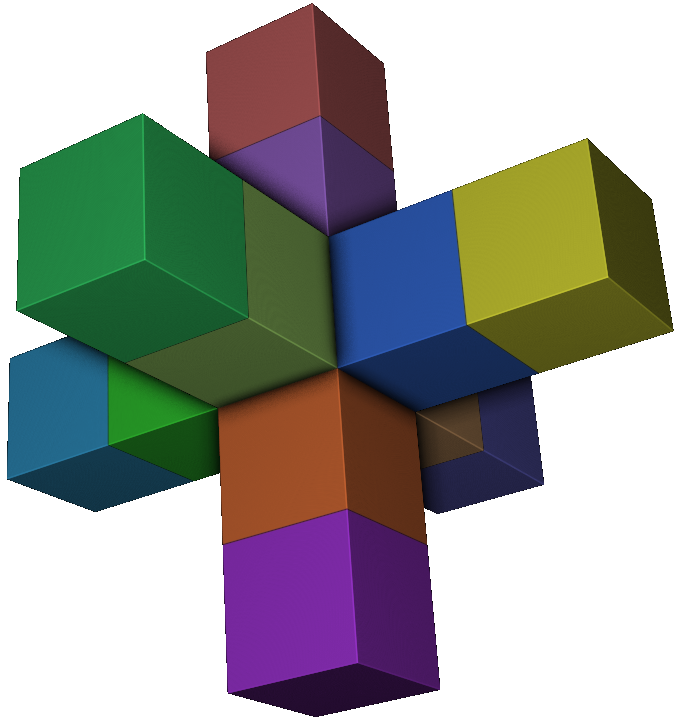
\includegraphics[width=.4\textwidth]{kr.png}
\hfill
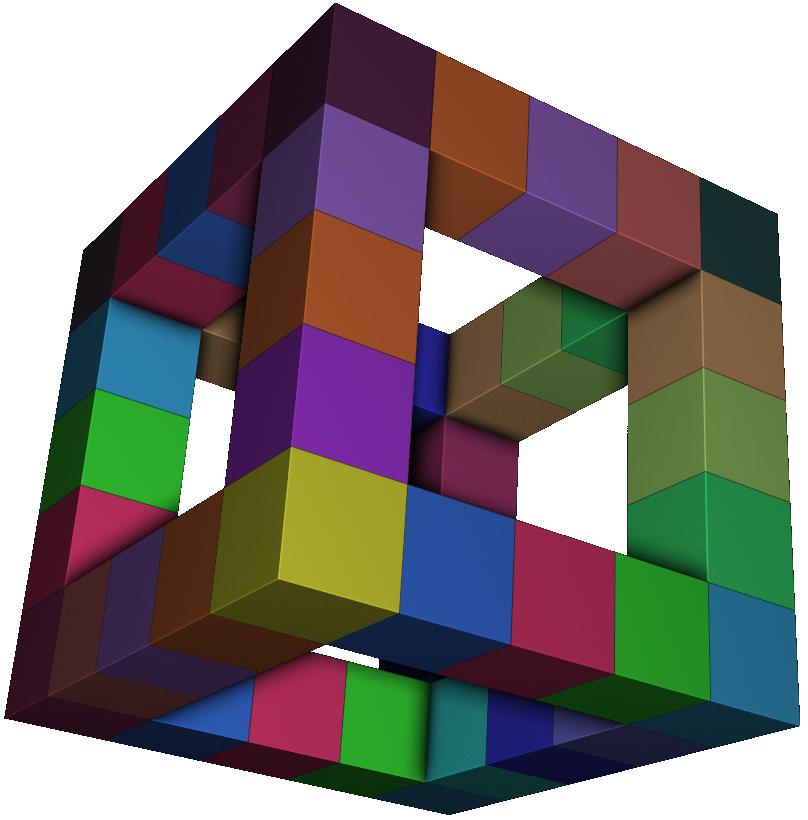
\includegraphics[width=.4\textwidth]{klb.png}
\qquad
\caption{ $P_0$ (слева) и $P_1$ (справа).}
\label{fig:5_1}
\end{figure}


{\bf 1.} Заметим, что $P_0\cap P_1=\0$, причем наименьшее расстояние $d(P_0,P_1)$ между точками этих множеств  равно 1/5.\smallskip

{\bf 2.} Множества $P_0$ и $P_1$ связны  и  инвариантны относительно группы симметрий куба $P$,  а их пересечения с гранями $W$ куба $P$ непусты. 
Обозначим через $W_0$   грань  $P$, лежащую в плоскости $\rr^2=\rr^2\times\{0\}$. 
Тогда $ D_0\cap\, \rr^2$ и $ D_1\cap\, \rr^2$ --- множества единиц, задающие фрактальные квадраты $K_0\cap W_0$ и $K_1\cap W_0$. 
Последние в силу симметрии конгруэнтны пересечениям $K_0$ и $K_1$ с любой из граней $W$ куба $P$.\smallskip

{\bf 3.} Пересечение множества $P_0$  с гранью $W_0$ куба $P$ --- центральный квадрат  на этой грани. 
Так как $ D_0\cap \rr^2=(2,2,0)$,  имеем $K_0\cap W_0=\{c_0\} $, где $c_0=(1/2,1/2,0)$ --- центр грани $W_0$. 
Значит в силу симметрии для каждой грани $W_i$,  $K_0\cap W_i=\{c_i\} $, где $c_i$ --- центр грани $W_i$. 
Поэтому множества $S_\xi(K_0)$ и $S_\eta(K_0)$ имеют непустое пересечение тогда и только тогда, когда кубы  $S_\xi(P)$ и $S_\eta(P)$ имеют общую грань, причем   единственной точкой пересечения при этом является центр этой общей грани.\smallskip

{\bf 4.} Ввиду {\bf 3} система сжимающих подобий $\eS_{ D_0}=\{S_\xi,\xi\in  D_0\}$ является системой с одноточечным пересечением. 
При этом  граф пересечений этой системы является деревом. 
Согласно \cite[Theorem 1.7]{FIP} фрактальный куб $K_0$ является дендритом.
Из строения графа пересечений системы $\eS_{D_0}$ следует, что  все точки ветвления $K_0$ имеют порядок 6.\smallskip

В свою очередь, фрактальный куб $ K_1$ --- это $ 5\times 5\times 5 $-версия губки Менгера.

\begin{figure}[h!]
\centering
\qquad
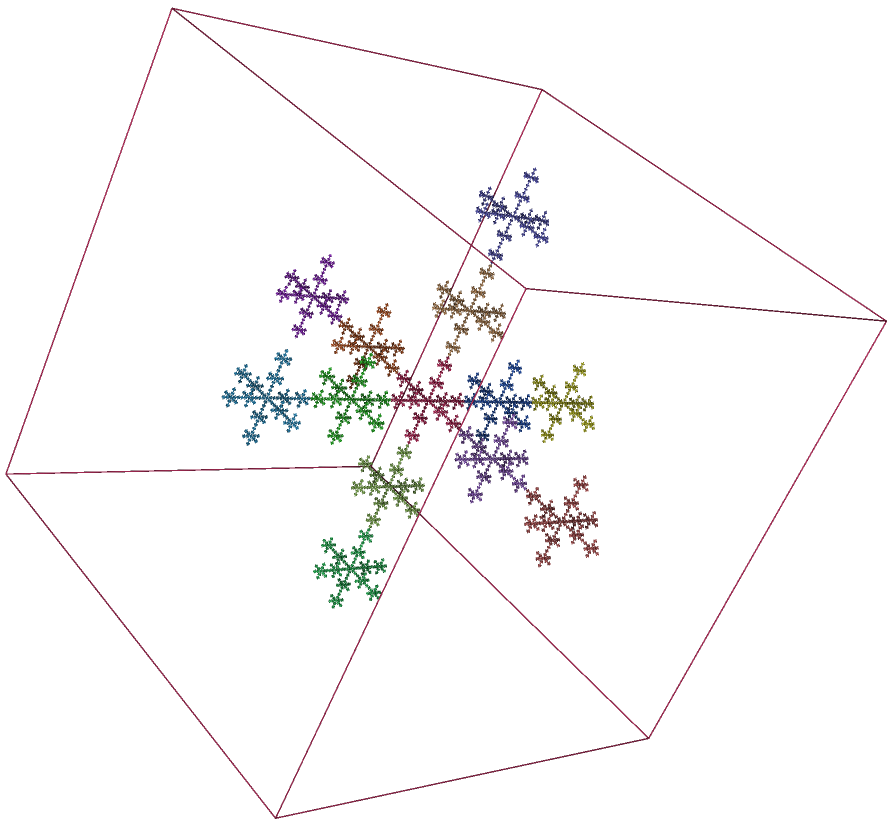
\includegraphics[width=.4\textwidth]{krr_a.png}
\hfill
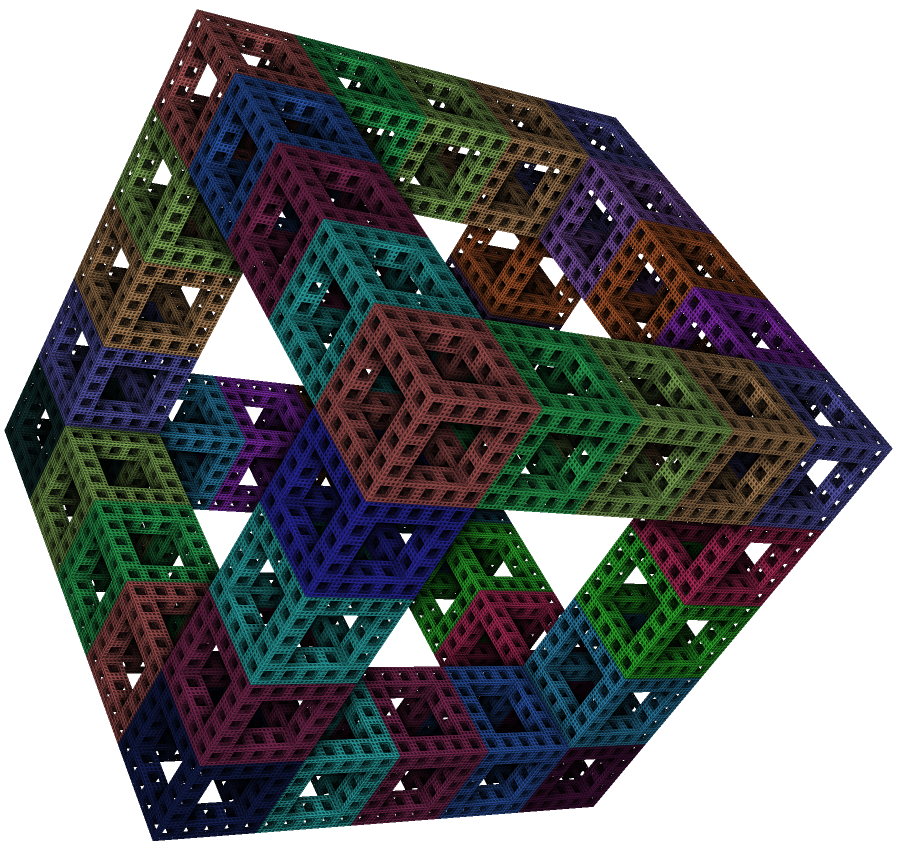
\includegraphics[width=.4\textwidth]{kl_a.png}
\qquad
\caption{Фрактальные кубы $K_0$ (слева) и $K_1$ (справа).}
\label{fig:5_2}
\end{figure}

{\bf Множество $ D$ и фрактальный куб $K$}.  
Определим $K$ как фрактальный куб (рис. \ref{fig:5_3}), множество единиц $D$ которого есть объединение непересекающихся множеств $D_0$  и  $D_1$. 
Оператор Хатчинсона $T$, порождающий фрактальный куб $K$, задается равенством $T(A)=T_0(A)\cup T_1(A)$. 
При этом множество $T(P)$ есть объединение непересекающихся связных множеств $P_0$  и $P_1$.

\begin{figure}[H]
\centering
\qquad
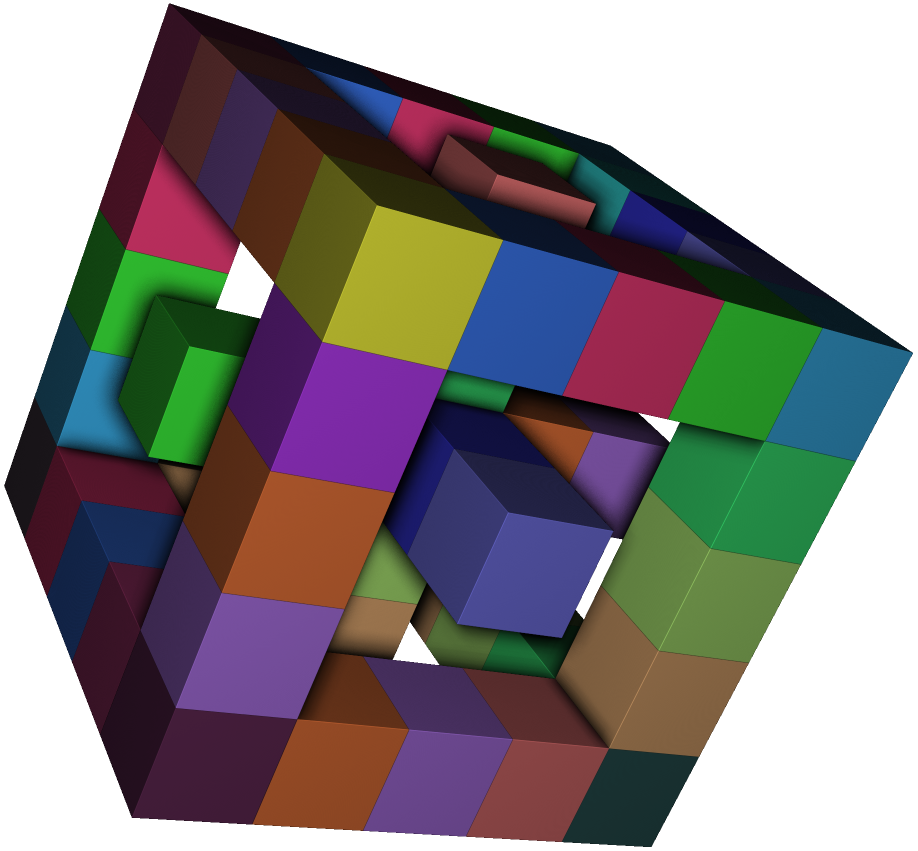
\includegraphics[width=.4\textwidth]{S.png}
\hfill
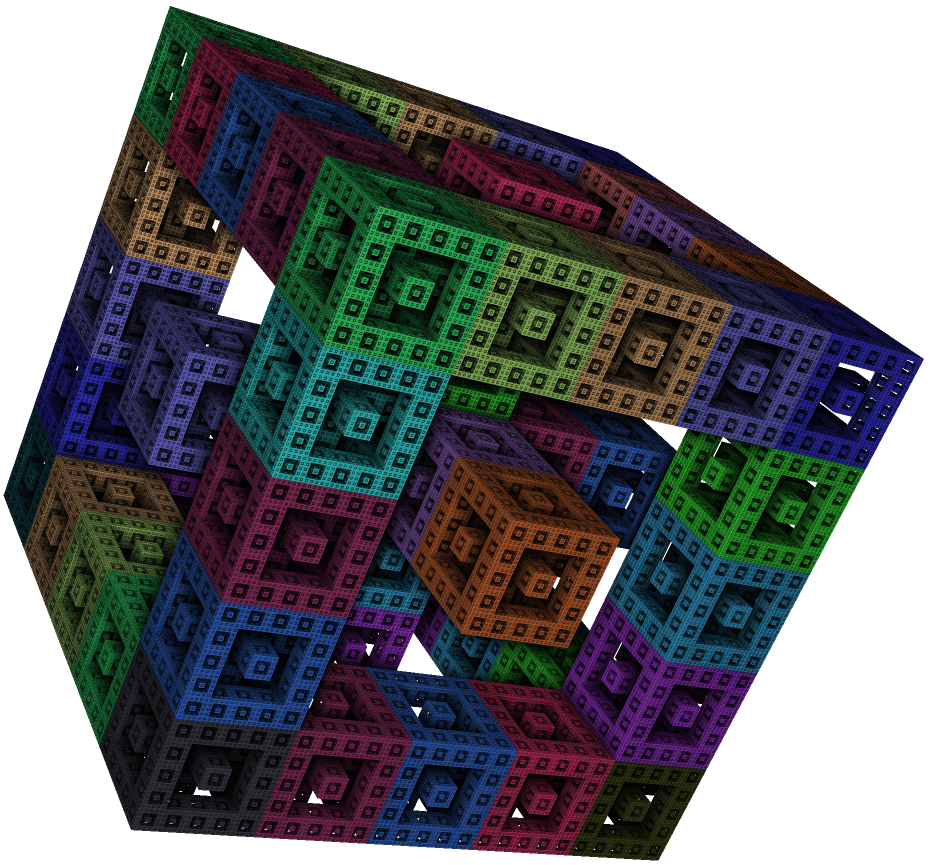
\includegraphics[width=.4\textwidth]{S_a.png}
\qquad
\caption{Множество $T(P)$ (слева) и фрактальный куб $K$ (справа)}
\label{fig:5_3}
\end{figure}



\section{Свойства множества $K$}
%\setcounter{equation}{0}

{\bf Индексное пространство для $K$}.
Поскольку фрактальный куб $K$ задается системой $\eS=\{S_\xi, \xi\in D\}$, то
для всякого $k$ элементы $\bar\xi=\xi_1\ldots\xi_k$ множества $ D^k$ мы будем называть {\it мультииндексами длины} $k$.
Множество всех мультииндексов мы обозначим через $ D^*=\bigcup_{k\in\nn} D^k$.

Мы будем называть {\em индексным пространством} системы $\eS$  пространство всех бесконечных строк  $\{\bmx=\xi_1\xi_2\xi_3…;\xi_i\in  D\}$, т.\,е. бесконечное произведение $D^\8$ конечных дискретных пространств $D$.

Запись $\bxi\sqsubset \bar\eta$ (соотв. $\bxi\sqsubset \bmx$) означает, что мультииндекс $\bxi$ является начальным подсловом в $\bar\eta$ (соотв. в $\bmx$).
Если не выполняется ни одно из соотношений $\bxi\sqsubset \bar\eta$, $ \bar\eta\sqsubset\bxi$, два мультииндекса называются несравнимыми. 
Символом $\bxi\wedge \bar\eta$ мы обозначаем максимальное общее начальное подслово в $\bxi$  и  $\bar\eta$. 
Запись $\bxi\bar\eta$ (соотв. $\bxi\bmx$) означает конкатенацию соответствующих слов или строк. 
Точно так же, если $A,B$ --- множества мультииндексов или строк, то $AB=\{\bxi\bar\eta: \bxi\in a,\bar\eta\in B\}$.   
Длина $k$ мультииндекса $\bar\xi=\xi_1\ldots\xi_k$ обозначается символом $|\bxi|$.

Каждый мультииндекс задает отображение $S_\bxi=S_{\xi_1\ldots\xi_k}=S_{\xi_1}\cdot\ldots\cdot S_{\xi_k}$. 
Поэтому $k$-е измельчение системы $\eS$ задается равенством $\eS^k=\{S_\bxi, \bxi\in  D^k\}$, а $k$-я степень оператора Хатчинсона системы $\eS$ задается равенством $T^k(A)=\bigcup_{\bxi\in D^k}S_\bxi(A)$.


Для каждой строки $\bmx=\xi_1\xi_2\xi_3\ldots\in  D^\8$ положим
\begin{equation}\label{pi}
\pi(\bmx)=\bigcap\limits_{n=1}^\8 S_{\xi_1\ldots\xi_n}(P)
\end{equation}
Формула \eqref{pi} задает единственную точку в множестве $K$ и тем самым определяет {\em индексное отображение} $\pi:D^\8\to K$.
\begin{lemma} \label{piD}
\begin{itemize}[nolistsep]
\item[{\rm (i)}] Для любого $\bxi\in D^*$, $\pi(\bxi D^\8)=S_\bxi(K);$
\item[{\rm (ii)}] Для $i=0,1$,\quad $\pi(D_i\times D^\8)=T_i(K);$
\item[{\rm (iii)}] Для любой строки $\bmx=\xi_1\xi_2\ldots.\in D^\8$ и  любого $\bx\in\rr^3$ , $\pi(\bmx)=\lim\limits_{k\to\8}S_{\xi_1\ldots\xi_k}(\bx).$ 
\end{itemize}
\end{lemma}

\begin{proof}
Из равенства \eqref{pi} следует, что для любых $\bxi\in D^*$, $\bmy\in D^\8$, $\pi(\bxi \bmy)=S_\bxi(\pi(\bmy))$. 
Так как $\pi(D^\8)=K$, получаем $\pi(\bxi D^\8)=S_\bxi(K)$.  
Аналогично, равенство $\pi(D_i\times D^\8)=\bigcup_{\xi\in D_i}S_{\xi}(K)$ дает (ii). 
Так как для любого $\bx\in\rr^3$   и для  $\bxi=\xi_1\ldots\xi_k$, расстояние $d(S_\bxi(\bx),S_\bxi(P))=d(x,P)/5^k $, переходя к пределу при $k\to\8$, получим (iii).
\end{proof}
  

{\bf Множество $Q$ и его точки $\cK_\bma$.}
Учитывая, что оператор $T$ удовлетворяет уравнению $T(A)=T_0(A)\cup T_1(A)$, мы рассмотрим систему сжимающих отображений $\Sa=\{ \tilde{T_0},\tilde{T_1}\}$ гиперпространства $C(\rr^3)$. 
Обозначим ее аттрактор через $Q$.

Так как $\Lip{\tilde T_i}=1/5$, аттрактор $Q$ системы $\Sa$ --- вполне несвязное компактное подмножество в $C(\rr^3)$. 
Более того, так как из включений $T_i(K)\IN K$ следует включение $\tT_0(C(K))\cup \tT_1(C(K))\IN C(K)$, множество $Q$ содержится в пространстве  $C(K)$ всех компактных подмножеств фрактального куба $K$.

Положим $I=\{0,1\}$. 
Каждому мультииндексу $\bal=\al_1\ldots\al_k\in I^k$  соответствует отображение $\tilde T_\bal=\tT_{\al_1}\cdot\ldots\cdot\tT_{\al_k}$ пространства $C(\rr^3)$ в себя, задаваемое равенством $ T_\bal(A)=T_{\al_1}\cdot\ldots\cdot T_{\al_k}(A)$. 
Положим $P_{\bar{\al}}=T_{\bar{\al}}(P).$

{\em Индексным пространством для системы $\Sa$} мы назовем множество $I^\8$. 
По теореме Хатчинсона, для каждой бесконечной строки $\bma=\al_1\al_2\ldots.\in I^\8$  и любого $A\in C(\rr^3)$ существует предел $\cK_\bma=\lim\limits_{m\to\8}T_{\al_1\ldots\al_m}(A)$, не зависящий от выбора   $A\in C(\rr^3)$. 
Тем самым  мы зададим {\em индексное отображение} $\sa:I^\8\to Q$ формулой $\sa(\bma)=\cK_\bma$.

В случае, когда $A=P$ (или $A=K$), множества $T_{\al_1\ldots\al_m}(P)=P_{\al_1\ldots\al_m}$ (соотв. $\cK_{\al_1\ldots\al_m}$) образуют последовательность вложенных компактов, поэтому предел последовательности $P_{\al_1\ldots\al_m}$ в метрике Хаусдорфа совпадает в их пересечением
\begin{equation}\label{sigma} 
\cK_\bma=\lim\limits_{m\to\8}P_{\al_1\ldots\al_m}=\bigcap\limits_{\bal\sqsubset \bma}P_\bal=\bigcap\limits_{\bal\sqsubset \bma}K_\bal.
\end{equation}

Если $\bma$ --- периодическая строка с периодом $\bar\al$, то множество $\cK_\bma\IN \rr^3$ удовлетворяет уравнению $\cK_\bma=T_{\bar{\al}}(\cK_\bma)$, и  в этом случае $\cK_\bma$ совпадает с аттрактором  $K_{\bar{\al}}$ оператора  $T_{\bar{\al}}$.


\begin{figure}[H]
\centering
\qquad
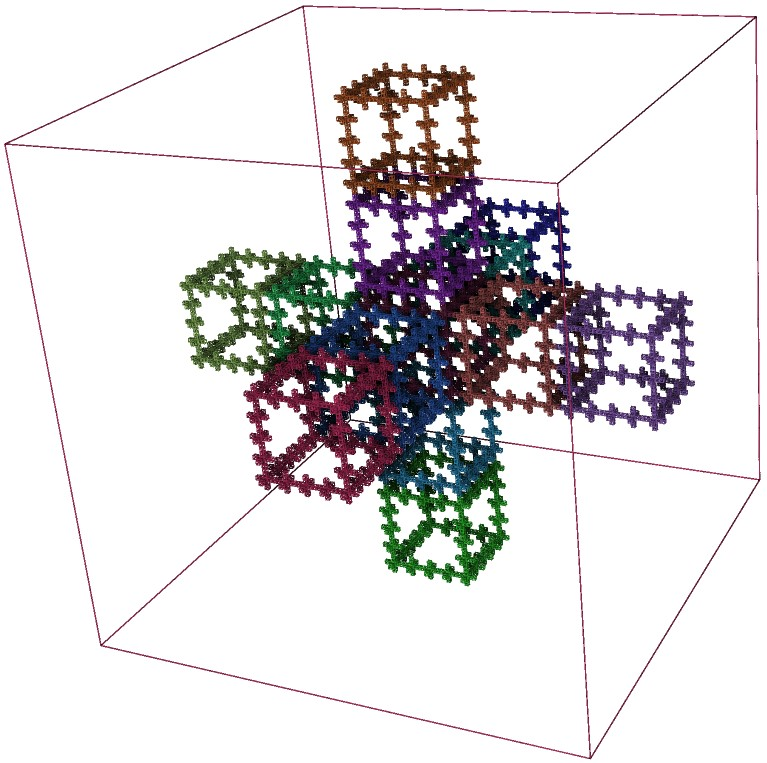
\includegraphics[width=.4\textwidth]{K01ar.jpg}
\hfill
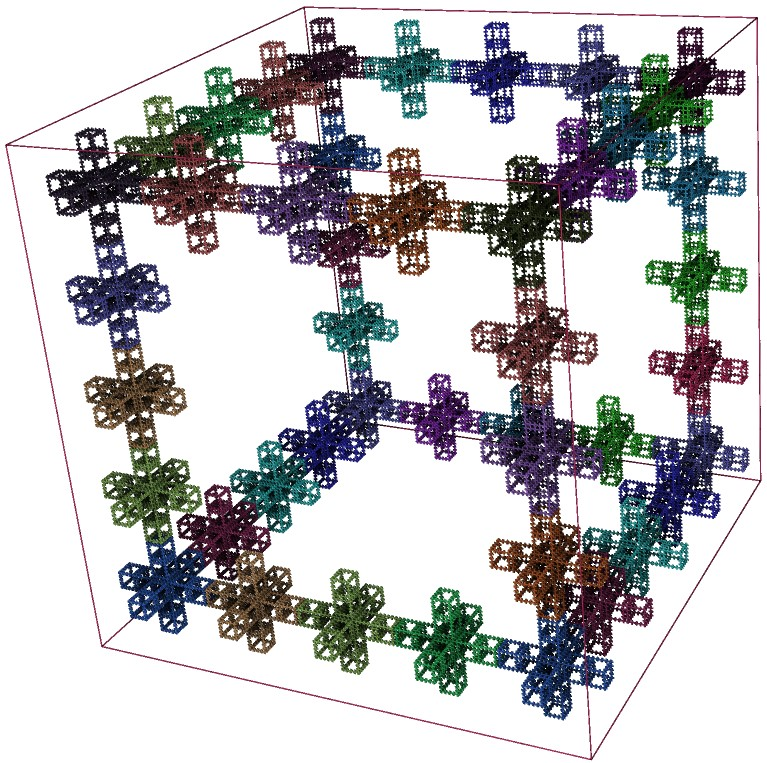
\includegraphics[width=.4\textwidth]{K10ar.jpg}
\qquad
\caption{Компоненты $K_{01}$ и $K_{10}$}
\label{fig:5_4}
\end{figure}


{\bf Сотношения между пространствами $D^\8$ и $I^\8$.} Пусть $\fy:D\to I$  ---  отображение, тождественно равное $0$ на   $D_0$ и равное $1$ на $D_1$. 
Для всякого $k\in\nn$ зададим отображение $\fy_k:D^k\to I^k$ равенством $\fy_k(\xi_1…\xi_k)=\fy(\xi_1)…\fy(\xi_k)$.
Для каждого мультииндекса  $\bal\in I^k$ положим $D_\bal=D_{\al_1}\times…\times D_{\al_k}$. 
Тогда для любого $\bal\in I^k$, $ \fy_k^{-1}(\bal)=D_\bal$.
При этом множество~$D^k$ есть дизъюнктное объединение подмножеств $D_\bal$ по всем $\bal\in I^k$.

Аналогично зададим отображение индексных пространств $\fy_\8: D^\8\to I^\8$ равенством $\fy_\8(\bmx)=\bma$, где  $\bmx=\xi_1…\xi_k\ldots$, а  $\bma=\fy(\xi_1)…\fy(\xi_k)\ldots$\,. 
Будучи произведением непрерывных отображений, $\fy_\8$ непрерывно.

Пусть $\bma=\al_1\al_2\ldots.$ и $D_\bma=\fy_\8^{-1}(\bma)$. 
Пространство $D_\bma$ есть бесконечное произведение компактных пространств $\prod_{i=1}^\8 D_{\al_i}$.
Поэтому множества $D_\bma$ компактны и $D^\8=\bigsqcup_{\bma\in I^\8}D_\bma$.
\begin{lemma}\label{svyaz}
\begin{itemize}[nolistsep]
\item[{\rm (i)}]  Для любого мультииндекса $\bar{\al}\in I^k, k\in\nn$ множество   $P_{\bar{\al}}$ связно\emph{;}
\item[{\rm (ii)}] Для любого $\bma\in\{0,1\}^\8$, множество $\cK_\bma$ связно\emph{;}
\item[{\rm (iii)}] $\pi(D_\bma)=\cK_\bma$ и $K=\bigcup_{\bma\in I^\8}\cK_\bma$.
\end{itemize}
\end{lemma}

\begin{proof}
(i) Множества $P_i$,  $i\in{0,1}$, обладают следующими  свойствами:\smallskip

(i1)  Множества $P_i$ инвариантны относительно симметрий куба $P$, в частности, пересечения~$P_i$ с любыми двумя противоположными гранями куба $P$ конгруэнтны относительно параллельного переноса одной грани в другую;\smallskip

(i2) любые два куба $(\xi+P)/5, (\eta+P)/5 \IN P_i$ с ребром длины $1/5$ в $P_i$ можно соединить путем, пересекающим только грани кубов из $P_i$ и не пересекающим их ребер.\smallskip

Если $\xi,\eta\in D_i$ таковы, что кубы $S_\xi(P), S_\eta(P)$ имеют общую грань, то $S_\xi(P_j)\cap S_\eta(P_j)$ имеет непустую внутренность.  
Поэтому для любых $i,j\in I$ множества $T_i(P_j)$ связны  и обладают теми же свойствами (i1) и (i2).

Рассуждая по индукции, мы получаем, что множества $T_{\al_1\ldots\al_k} (P_i)$ связны и наследуют  свойства (i1), (i2).\smallskip

(ii) Так как $\cK_\bma$ --- пересечение убывающей по включению последовательности связных компактных множеств $P_{\al_1\ldots.\al_m},$  множество $\cK_\bma$ также компактно и связно и обладает свойствами (i1), (i2).\smallskip

(iii) Множество $D_\bma$ есть пересечение убывающей последовательности компактов
$D_{\al_1\ldots\al_k}\times D^\8$. Согласно лемме  \ref{piD} $\pi(D_{\al_1\ldots\al_k}\times D^\8)=K_{\al_1\ldots\al_k} $,  поэтому $\pi(D_\bma)\IN \cK_\bma$. Поскольку $K=\pi(D^\8)=\bigcup_{\bma\in I^\8}\pi(D_\bma)$, то $K=\bigcup_{\bma\in I^\8}\cK_\bma$.
\end{proof}


Из конструкции  множеств $ D_0, D_1$ следует, что хаусдорфово расстояние между множествами $d_H(P_0,P_1)=2\sqrt{2}/5$, $d_H(P,P_i)\le 2\sqrt{2}/5$, в то время как минимальное расстояние $d( P_0, P_1)$ между точками этих множеств равно 1/5. 
Отсюда мы получаем следующие оценки.
\begin{lemma}\label{dhf}
Пусть $\bar{\al}, \bar{\be}\in I^*$ --- несравнимые мультииндексы.
Тогда
$$P_{\bar{\al}}\cap P_{\bar{\be}}=\0,\ \ 
 =d_H(P_{\bar{\al}},P_{\bar{\be}})<{3\sqrt5}/{5^{|\bar{\al}\wedge\bar{\be}|}}\ \  
\text{и}\ \ d(P_{\bar{\al}},P_{\bar{\be}})\geq{1}/{5^{|\bar{\al}\wedge\bar{\be}|+1}}.$$
\end{lemma}

\begin{proof}
Если $\al_1\neq\be_1$, то $P_{\bar{\al}}\IN P_{\al_1}, P_{\bar{\be}}\IN P_{\be_1},$ следовательно,
\begin{equation} \label{df}
d_H(P_{\bar{\al}},P_{\bar{\be}})\leq d_H(P_{\bar{\al}},P_{\al_1})+d_H(P_{\al_1},P_{\be_1})+d_H(P_{\bar{\be}},P_{\be_1}) \leq \frac{2\sqrt2}{25}+\frac{2\sqrt2}{5}+\frac{2\sqrt2}{25} < \frac{3\sqrt2}{5}
\end{equation}
и $d(P_{\bar{\al}},P_{\bar{\be}})\geq d(P_{\al_1},P_{\be_1})=1/5.$
Заметим, что $d_H(P_{\sa\bar{\al}}, P_{\sa\bar{\be}})={d_H(P_{\bar{\al}}, P_{\bar{\be}})}/{5^{|\sa|}}$ и $d(P_{\sa\bal},P_{\sa\bar\be})={d(P_{\bal},P_{\bar\be})}/{5^{|\sa|}}$, из чего вытекает утверждение леммы.
\end{proof}

Пусть $\bma=\al_1\al_2\al_3\ldots\in I^\8.$ 
Заметим, что $\cK_{\bma}=\bigcap_{k=1}^\8 P_{\al_1\ldots\al_k} $ есть пересечение убывающей последовательности множеств $P_{\al_1\ldots\al_k}$. 
Тогда, переходя к пределу при $k\to\8$ в неравенстве~\eqref{df} и в дальнейших рассуждениях леммы \ref{dhf}, получим\smallskip

{\bf Утверждение.}\ \
{\it Для любых $\bma, \bmb\in I^\8$}
$$\frac{1}{5^{|\bma\wedge\bmb|}+1} \leq d_H(\cK_{\bma},\cK_{\bmb}) < \frac{3\sqrt5}{5^{|\bma\wedge\bmb|+1}},$$ и
$$d(\cK_{\bma},\cK_{\bmb})\geq \frac{1}{5^{|\bma\wedge\bmb|+1}}.\eqno\square$$

\begin{proof}[теоремы \ref{GGM}]
По лемме \ref{svyaz} каждое множество $\cK_\bma$ связно и компактно. 
Для каждого $k$ множества $P_{\bar\al}, \bar\al\in I^k$ образуют конечное покрытие $K$ попарно непересекающимися континуумами. 
При этом из включения $K_\bal:=T_\bal(K)\IN P_\bal$ следует что $K_\bal= K\cap P_\bal$. 
Поэтому для любых $\bal\in I^*$, множества $K_\bal$ открыто-замкнуты в $K$. 
Поэтому  $\{K_\bal,\bal\sqsubset\bma\}$~--- фундаментальная система открыто-замкнутых окрестностей множества $\cK_\bma$, и каждое из множеств $\cK_\bma$ является связной компонентой $K$. 
При этом $K=\bigsqcup\limits{\bma\in I^\8}\cK_\bma$.

Пусть $x_\bma, x_\bmb$ --- точки канторова множества $C_{1/5}$ с адресами $\bma, \bmb$. 
Они удовлетворяют неравенству
$$3\cdot5^{-(|\bar{\al}\wedge\bar{\be}|+1)} < d(x_\bma, x_\bmb) < 5^{-(|\bar{\al}\wedge\bar{\be}|)}.$$
В то же время для точек $\cK_{\bma},\cK_{\bmb}\in Q$ выполняется неравенство
\begin{equation}\label{dva} 
5^{-(|\bar{\al}\wedge\bar{\be}|+1)} < d_H(\cK_{\bma},\cK_{\bmb}) < 3\sqrt5\cdot 5^{-(|\bar{\al}\wedge\bar{\be}|+1)}.
\end{equation}

Из неравенства \eqref{dva} получим
\begin{equation}\label{tri} 
d(x_\bma, x_\bmb)/5<d_H(\cK_{\bma},\cK_{\bmb})< \sqrt5\cdot d(x_\bma, x_\bmb).
\end{equation}

Пусть $\psi:C_{1/5}\to Q$  задается формулой $\psi(x_\bma)=\cK_\bma$. Согласно \eqref{tri}  $\psi$  --- билипшицев гомеоморфизм между $C_{1/5}$ и $Q$. 
Если $f_0(x)=x/5$, $f_1(x)=x/5+4/5$  --- отображения в $\rr$, порождающие $C_{1/5}$, то $\psi\cdot f_i=\tilde T_i\circ\psi$. 
Поэтому гомеоморфизм $\psi$ индуцирует изоморфизм самоподобных структур на $C_{1/5}$ и $Q$. 
\end{proof}

\begin{proof}[теоремы 2]
Для любой компоненты $\cK_\bma$ расширение $\cK_\bma+\zz^3$ связно, поскольку  пересечения $\cK_\bma$ с любыми двумя противоположными гранями куба $P$ конгруэнтны относительно параллельного переноса одной грани в другую.
Поскольку такое рассширение получено путем объединения $\mathbb{Z}^3$-сдвигов компоненты $\cK_\bma$, то $\cK_\bma+\zz^3$ инвариантно относительно $\mathbb{Z}^3$-сдвигов. 
Значит, $H=K+\zz^k$ есть несчетное объединение неограниченных компонент, каждая из которых инвариантна относительно $\mathbb{Z}^3$-сдвигов.

Далее, поскольку $K=\bigcap_{k=1}^\8 T^k(P)$ есть пересечение убывающей по включению последовательности компактов, то множество $P\mmm K=\bigcup_{k=1}^\8 P\mmm T^k(P)$ объединение возрастающей последовательности открытых подмножеств из $P$, каждое из которых связно. 
Поэтому $P\mmm K$ связно. С другой стороны, поскольку пересечения $P\mmm K$ с противоположными гранями куба~$P$ конгруэнтны, то множество $H^c=P\mmm K +\zz^3$ связно. 
\end{proof}



\section{Размерности компонент}
%\setcounter{equation}{0}

Пусть $\bma=\al_1 \al_2 \ldots\in I^\8.$ 
Для любого $k \in\nn$ {\em плотностью единиц} в начальном подслове $\al_{1}\ldots\al_{k}$ мультииндекса $\bma$ мы назовем число $\la_{k}(\bma)=k^{-1}\sum_{i=1}^k\al_i$. 
Положим $\overline{\la}_\bma=\limsup\limits_{k\to\8}{\la_{k}(\bma)}$,\ $\underline{\la}_\bma=\liminf\limits_{k\to\8}{\la_{k}(\bma)}$ и, если $\underline{\la}_\bma=\overline\la_\bma$, мы пишем $\la_\bma=\lim\limits_{k\to\8}{\la_{k}(\bma)}.$
 Если $\bma$ --- предпериодическая строка с длиной периода $p$, то $\la_\bma$ равна плотности единиц в любом подслове $\bar\be$ длины $p$ из периодической части строки $\bma$.\smallskip

Справедлива  следующая  теорема.
\begin{theorem}\label{tdim}
Для любого $\bma\in I^\8$
$$\overline{\dim}_B(\cK_\bma)=(1-\overline\la_\bma)\log_513+\overline\la_\bma\log_544$$
$$\dim_H(\cK_\bma)=\underline{\dim}_B(\cK_\bma)=(1-\underline{\la}_\bma)\log_513+\underline{\la}_\bma\log_544$$

Если строка $\bma$ --- предпериодическая, то $\cK_\bma$ имеет положительную меру Хаусдорфа в размерности $\dim_H(\cK_\bma)$.
\end{theorem}

\begin{proof}
Пусть $\bal\sqsubset \bma, |\bal|= k$ и $\sum_{i=1}^k\al_i=m$. 
Множество $P_\bal$ состоит из $\#D_\bal=13^{k-m}44^m$ кубов с ребром $\da_k=5^{-k}$, и эти кубы образуют $\da_k$-покрытие $\cK_\bma$. 
Обозначая  $a=\log_513$ и $b=\log_544$, получим $-{\ln N_{\da_k}}/{\ln\da_k}=(1- \la_{k}(\bma))a + \la_{k}(\bma)b$, поэтому 
\begin{equation}
\liminf\limits_{k\to\8}\dfrac{-\ln N_{\da_k}}{\ln\da_k}= a+(b-a)\underline\la(\bma) 
\mbox{\quad  и  \quad}
\limsup\limits_{k\to\8}\dfrac{-\ln N_{\da_k}}{\ln\da_k}= a+(b-a)\overline\la(\bma),
\end{equation}
что и дает формулы для верхней и нижней клеточной размерности.

Для $p$-периодического $\bma=\overline{\al_1\al_2\ldots\al_p}\in I^\8$,  $\underline{\la}_\bma=\overline{\la}_\bma$, и $\overline{\dim}_B(\cK_\bma) = \underline{\dim}_B(\cK_\bma) = \dim_B(\cK_\bma)$.
В силу уравнения $\cK_\bma=T_{\al_1\al_2\ldots\al_p} (\cK_\bma)$ множество $\cK_\bma$ является аттрактором системы $\{S_\bxi; \bxi\in D_{\al_1\al_2\ldots\al_p}\}$, удовлетворяющей условию открытого множества (OSC).  
Поэтому~(см.~\cite[Theorem 9.3, p.~118]{Fal}) $\dim_H (\cK_\bma)= \dim_B (\cK_\bma)$ и $\cK_\bma$ имеет конечную положительную меру  в этой размерности.

Последнее верно и для предпериодических $\bma$. Если $\bma=\bar\be\bmb$, где $\bar\be$ --- конечное подслово  и  $\bmb$~--- периодическая часть, то  $\cK_\bma=T_{\bar\be}(\cK_\bmb)$. Тогда $\dim_H (\cK_\bma)= \dim_H (\cK_\bmb)$. 
Так как $\la(\bmb)=\la(\bma)$, имеем $\dim_H (\cK_\bma)=a+(b-a)\la(\bma)$.

Теперь докажем, что $\dim_H(\cK_\bma)=\underline{\dim}_B(\cK_\bma)$ для любой строки $\bma$.
Пусть $\bma=\al_1\al_2\ldots$. Для каждого $k$  будем обозначать   $k$-й  остаток последовательности как $\bma_k=\al_{k+1}\al_{k+2}\ldots$.


Зададим вероятностную меру $\mu_\bma$ на пространстве $D_{\bma}$ как произведение равномерных вероятностных мер на сомножителях $D_{\al_i}$. Для каждого $k\in\nn$ и $\bxi\in D_{\al_1\ldots\al_k}$,
 \[\mu(\bxi D_{\bma_k})=(\#D_{\al_1\ldots\al_k})^{-1}=5^{-k(a+\la_k(\bma)\cdot(b-a))} .\]

Пусть $\La(t)=5^{-(a+t(b-a))}$. Функция $\La(t)$ убывает на $[0,1]$, и $\La(0)=1/13$, а  $\La(1)=1/44$.

Зададим меру $\tilde\mu$ c носителем в $\cK_\bma$, положив для всякого $A\IN P$, $\tilde\mu_\bma(A)=\mu_\bma(\pi^{-1}(A\cap \cK_\bma))$. Покажем, что для этой меры выполняется принцип распределения масс.

Пусть $B$ --- шар, такой что
\begin{equation}\label{ner}
{\sqrt{3}}\cdot 5^{-n-1}<|B|\le{\sqrt{3}}\cdot 5^{-n}.
\end{equation}
Тогда $B$ содержится не более, чем в 27 кубах со стороной $5^{-n}$. 
Поэтому для множества $B\cap \cK_\bma$  его прообраз $\pi^{-1}(B\cap \cK_\bma)$ содержится не более чем в 27 множествах  $\xi_1\ldots \xi_n D_{\bma_n}$, мера каждого из которых равна $\La(\la_n)^n$.

Отсюда следует неравенство $\tilde\mu(B)<27\La(\la_n)^n$.

По определению нижней плотности $\underline{\la}_\bma$, для любого $\nu<\underline{\la}_\bma$ существует такое $N\in\nn$, что при $n>N$, $\la_n(\bma) > \nu$. 
Тогда $\La(\nu)>\La(\la_n)$  и поэтому  $\tilde\mu(B)<27\La(\nu)^n$.

Из левой части неравенства \eqref{ner} получаем, что $n>\log_5(\sqrt{3}/(5|B|))$.
Тогда 
\begin{equation}
\tilde\mu(B)<27 \La(\nu)^{\log_5(\sqrt{3}/(5|B|))}=L\cdot|B|^{-\log_5{\La(\nu)}} =L\cdot |B|^{a+\nu(b-a)},
\end{equation}
где $L=27\cdot(5^{-1}\sqrt{3})^{\log_5{\La(\nu)}}$ --- положительная постоянная.

Согласно принципу распределения масс \cite[Mass distribution Principle~4.2, p.55]{Falconer2004}, $\dim_H(\cK_\bma)\geqslant a+\nu(b-a)$ для любого $\nu<\underline{\la}_\bma$.
Следовательно, $\dim_H(\cK_\bma)\geqslant  a+(b-a)\underline\la(\bma) =\underline{\dim}_B(\cK_\bma)$.

Поскольку  для любого непустого компакта $K\IN\rr^d$ справедливо неравенство $\dim_H(K)\leqslant\underline{\dim}_B(K)$ \cite[(3.17), p.~43]{Falconer2004}, мы получаем, что $\dim_H( \cK_\bma)=\underline{\dim}_B( \cK_\bma)$.
\end{proof}

\begin{remark} 
Для произвольного $\bma\in I^\8$ нельзя утверждать ни положительность, ни конечность меры Хаусдорфа множества $\cK_\bma$ в его размерности. 
Если в строке $\bma=\al_1\al_2\ldots$ индексы $\al_i=0$ при  $i=n(n+1)/2$ и $\al_i=1$ в остальных случаях, то $\dim_H(\cK_\bma)=b$, причем хаусдорфова мера $H^b(\cK_\bma)=0$.
Если же $\al_i=1$ при  $i=n(n+1)/2$ и $\al_i=0$ в остальных случаях,то $\dim_H(\cK_\bma)=a$, причем хаусдорфова мера $H^a(\cK_\bma)=\8$.
\end{remark}
 
 
 
 